%************************************************
\chapter{Theory}
\label{chp:theory}
%************************************************

\textit{In this chapter relevant theory is presented; both mathematical models and algorithms. To model the road network a graph representation will be used, further we present an extended graph representation. We also introduce theory on the HMM and the Viterbi algorithm which is used for the map generation process.}

%========================================================================%
\section{Graph}
\label{chp:theory.sec:graph}
%========================================================================%

To describe the structure of a network a \textit{graph} is often used. It describes the connections, or edges, $\mathcal{E}$, between the vertices, or nodes, $\mathcal{V}$. Furthermore, an adjacency matrix $W$ describes the weights on the edges. More formally we define a graph as

\begin{equation}
    \mathcal{G} = (\mathcal{V, E}, W). 
\end{equation}

A graph with $n$ nodes is therefore represented by $\mathcal{V} = \{1, 2, ..., n\}$ and corresponding adjacency matrix $W \in \mathbb{R}_+^{n\times n}$. Having two nodes $i, j \in \mathcal{V}$, an edge $(i,j) \in \mathcal{E}$ is said to exist if and only if $W_{ij} > 0$. A graph $\mathcal{G}$ can be both undirected or directed. If it is undirected the adjacency matrix $W$ is symmetric, which means having the same weight in both directions between two nodes $W_{ij} = W_{ji}$. Furthermore, a graph is said to be unweighted if and only if $W_{ij}\in\{0,1\}$ for all $i,j \in \mathcal{V}$. For the application in this master's thesis a directed, weighted graph will be used. In figure \ref{fig:theory/graph} an illustration of a directed graph is presented. This graph is directed since at least one pair of nodes has only one edge connecting them. Between node $i,j \in \mathcal{V}$ there is one edge $(i,j)$, whereas for nodes $i',j' \in \mathcal{V}$ there is one edge in each direction, $(i',j') \in \mathcal{E}$ and $(j',i') \in \mathcal{E}$ \citep{giacomo}.
\iffalse
\begin{figure}[H]
    \centering
    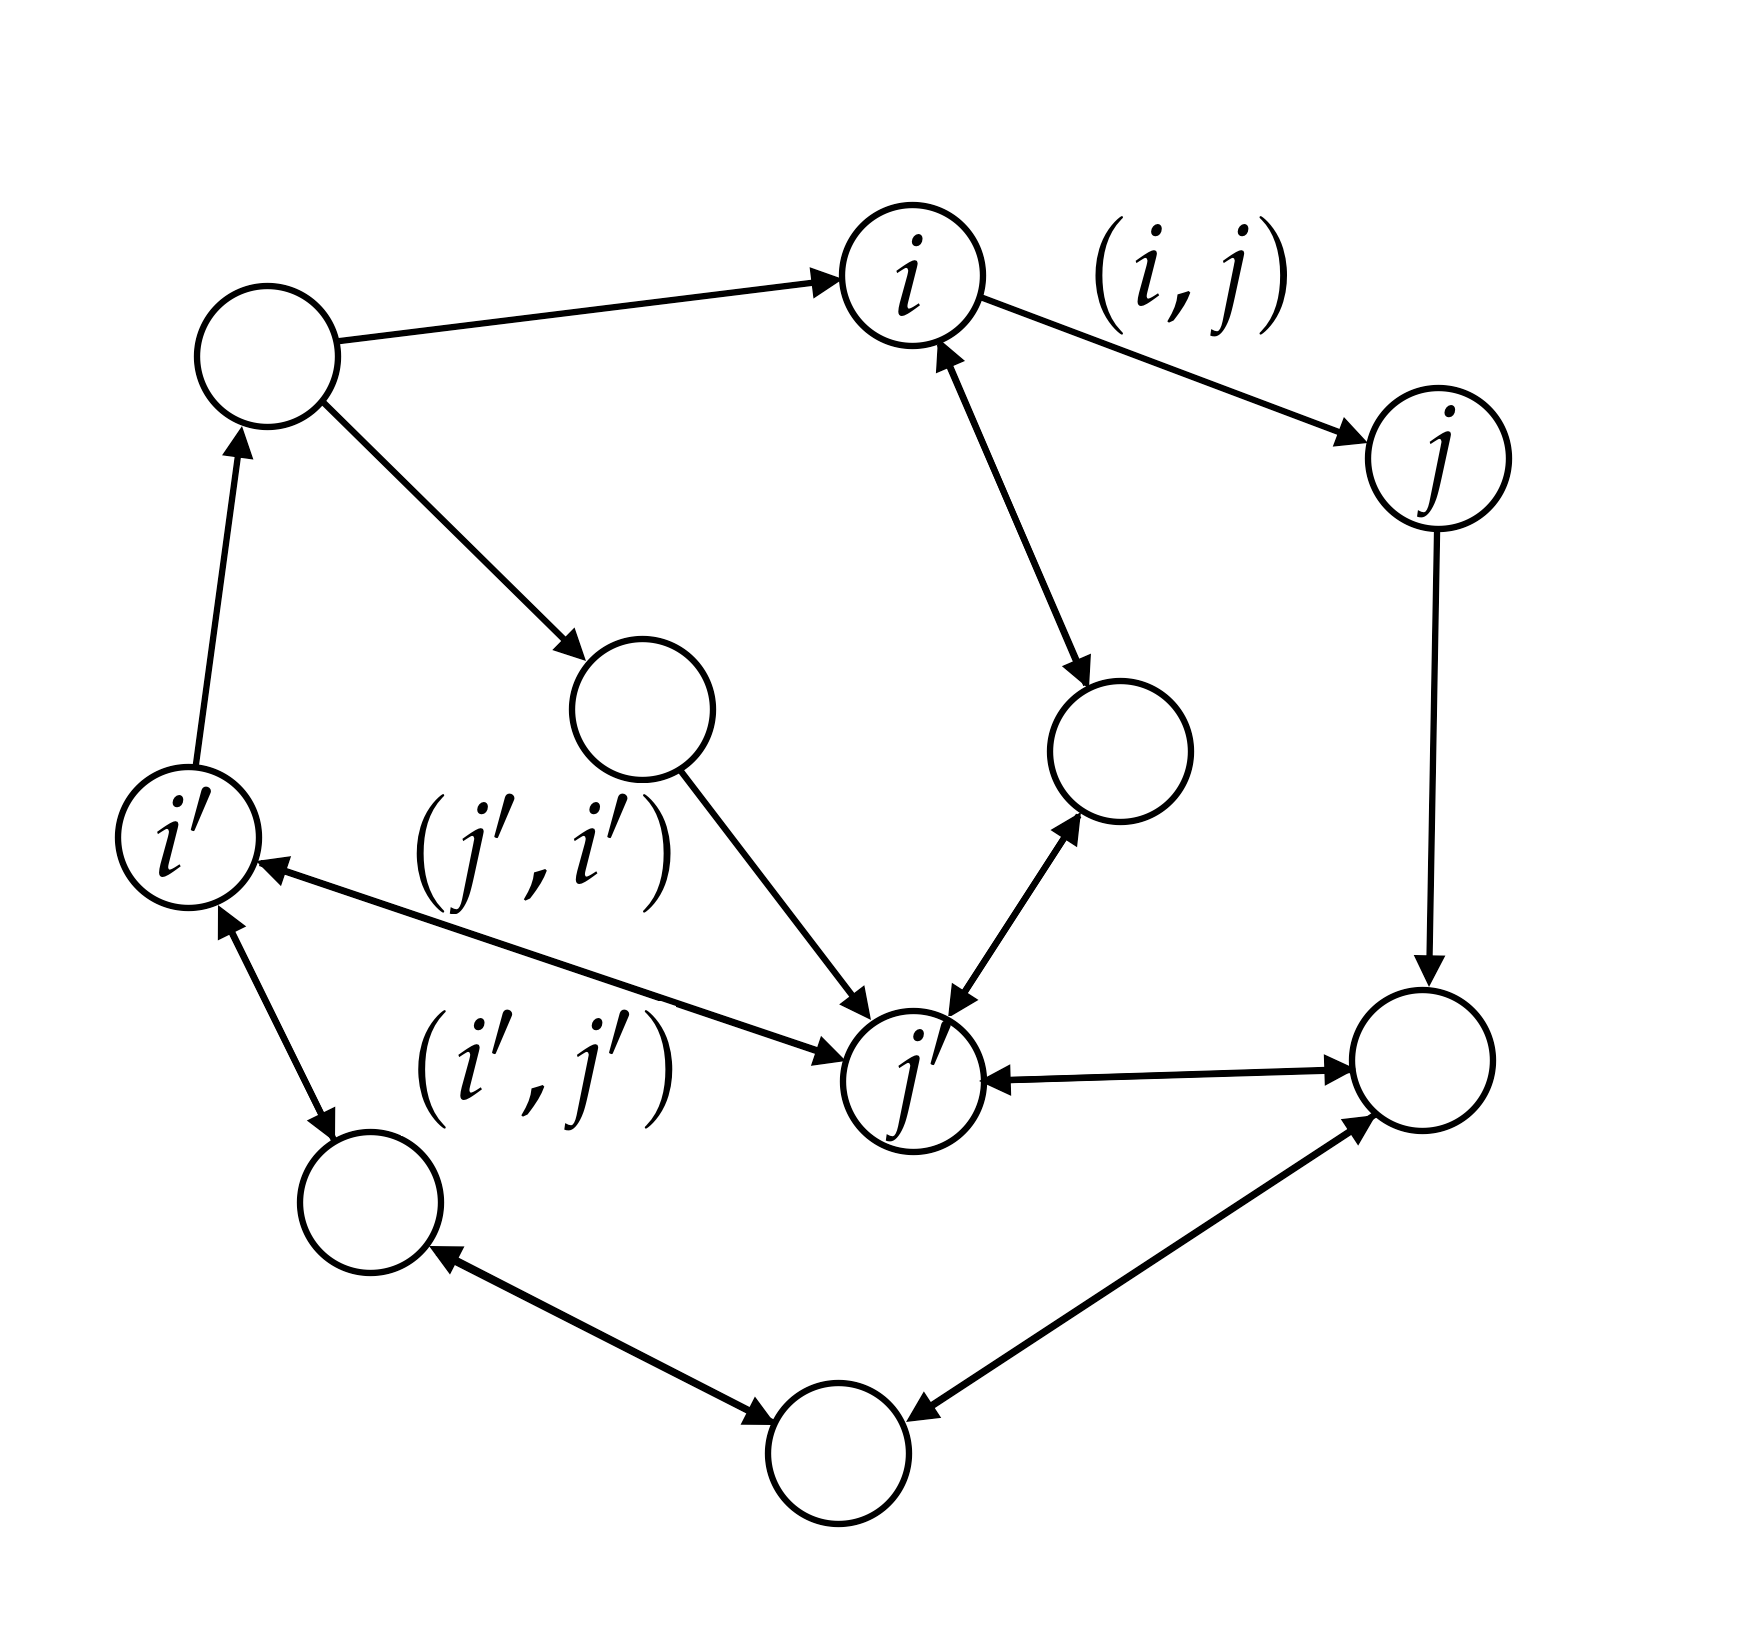
\includegraphics[width=0.6\linewidth]{Figures/Theory/graph_better.png}
    \caption{A directed graph.}
    \label{fig:theory/graph}
\end{figure}
\fi
\begin{figure}[H]%
 \centering
 \subfloat[\textit{A directed graph.}]{{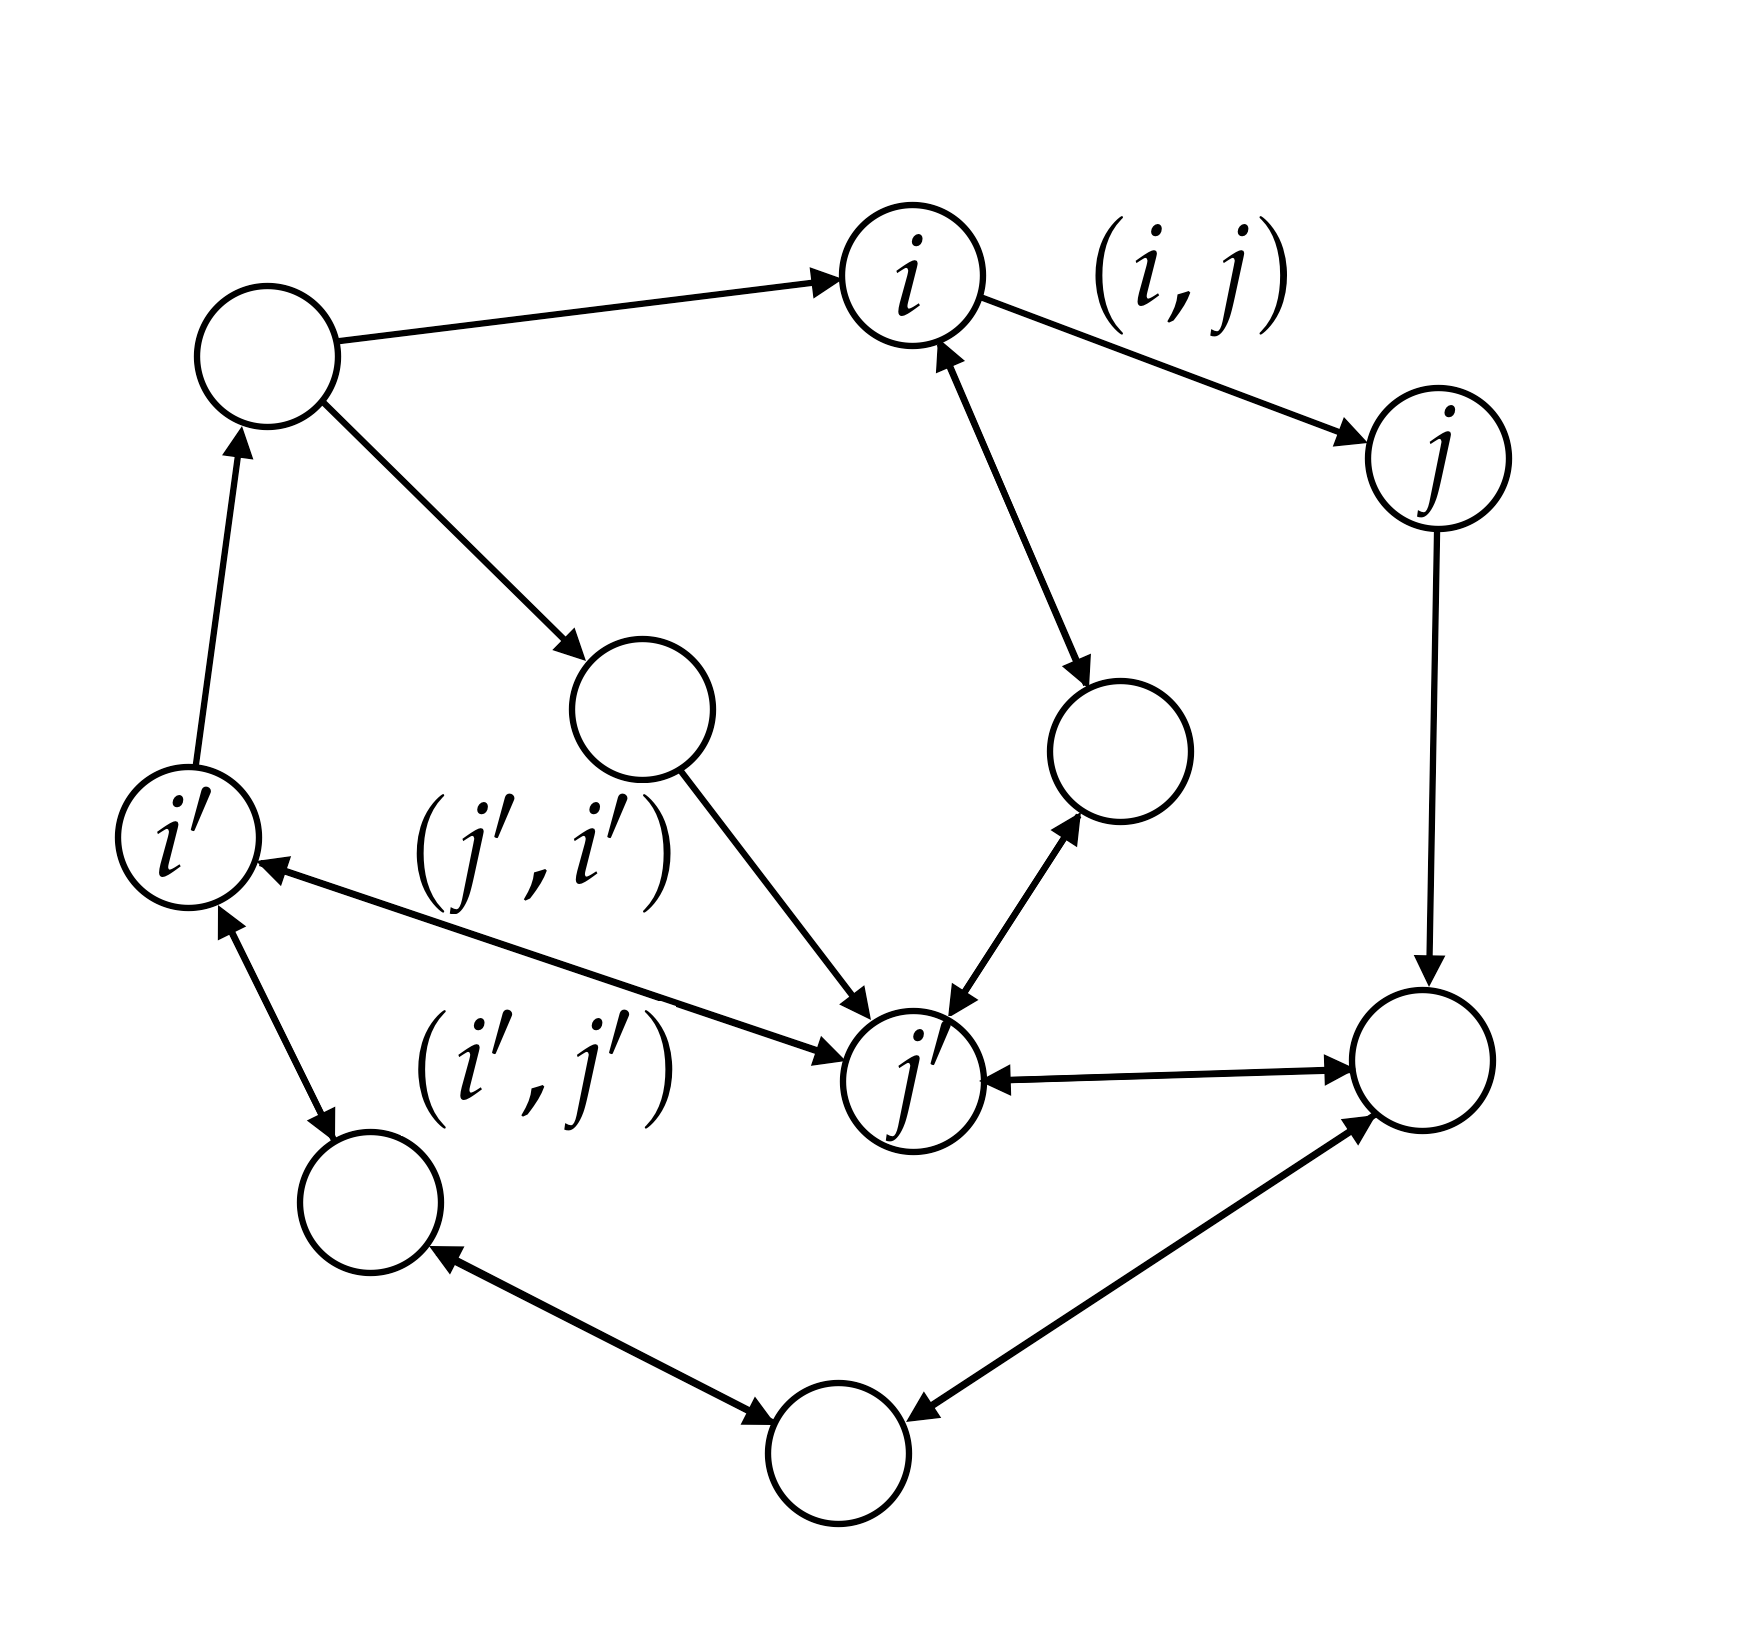
\includegraphics[width=0.7\linewidth]{Figures/Theory/graph_better.png}\label{fig:theory/graph} }}% 
 
 \subfloat[\textit{Segments and edges using the extended representation.}]{{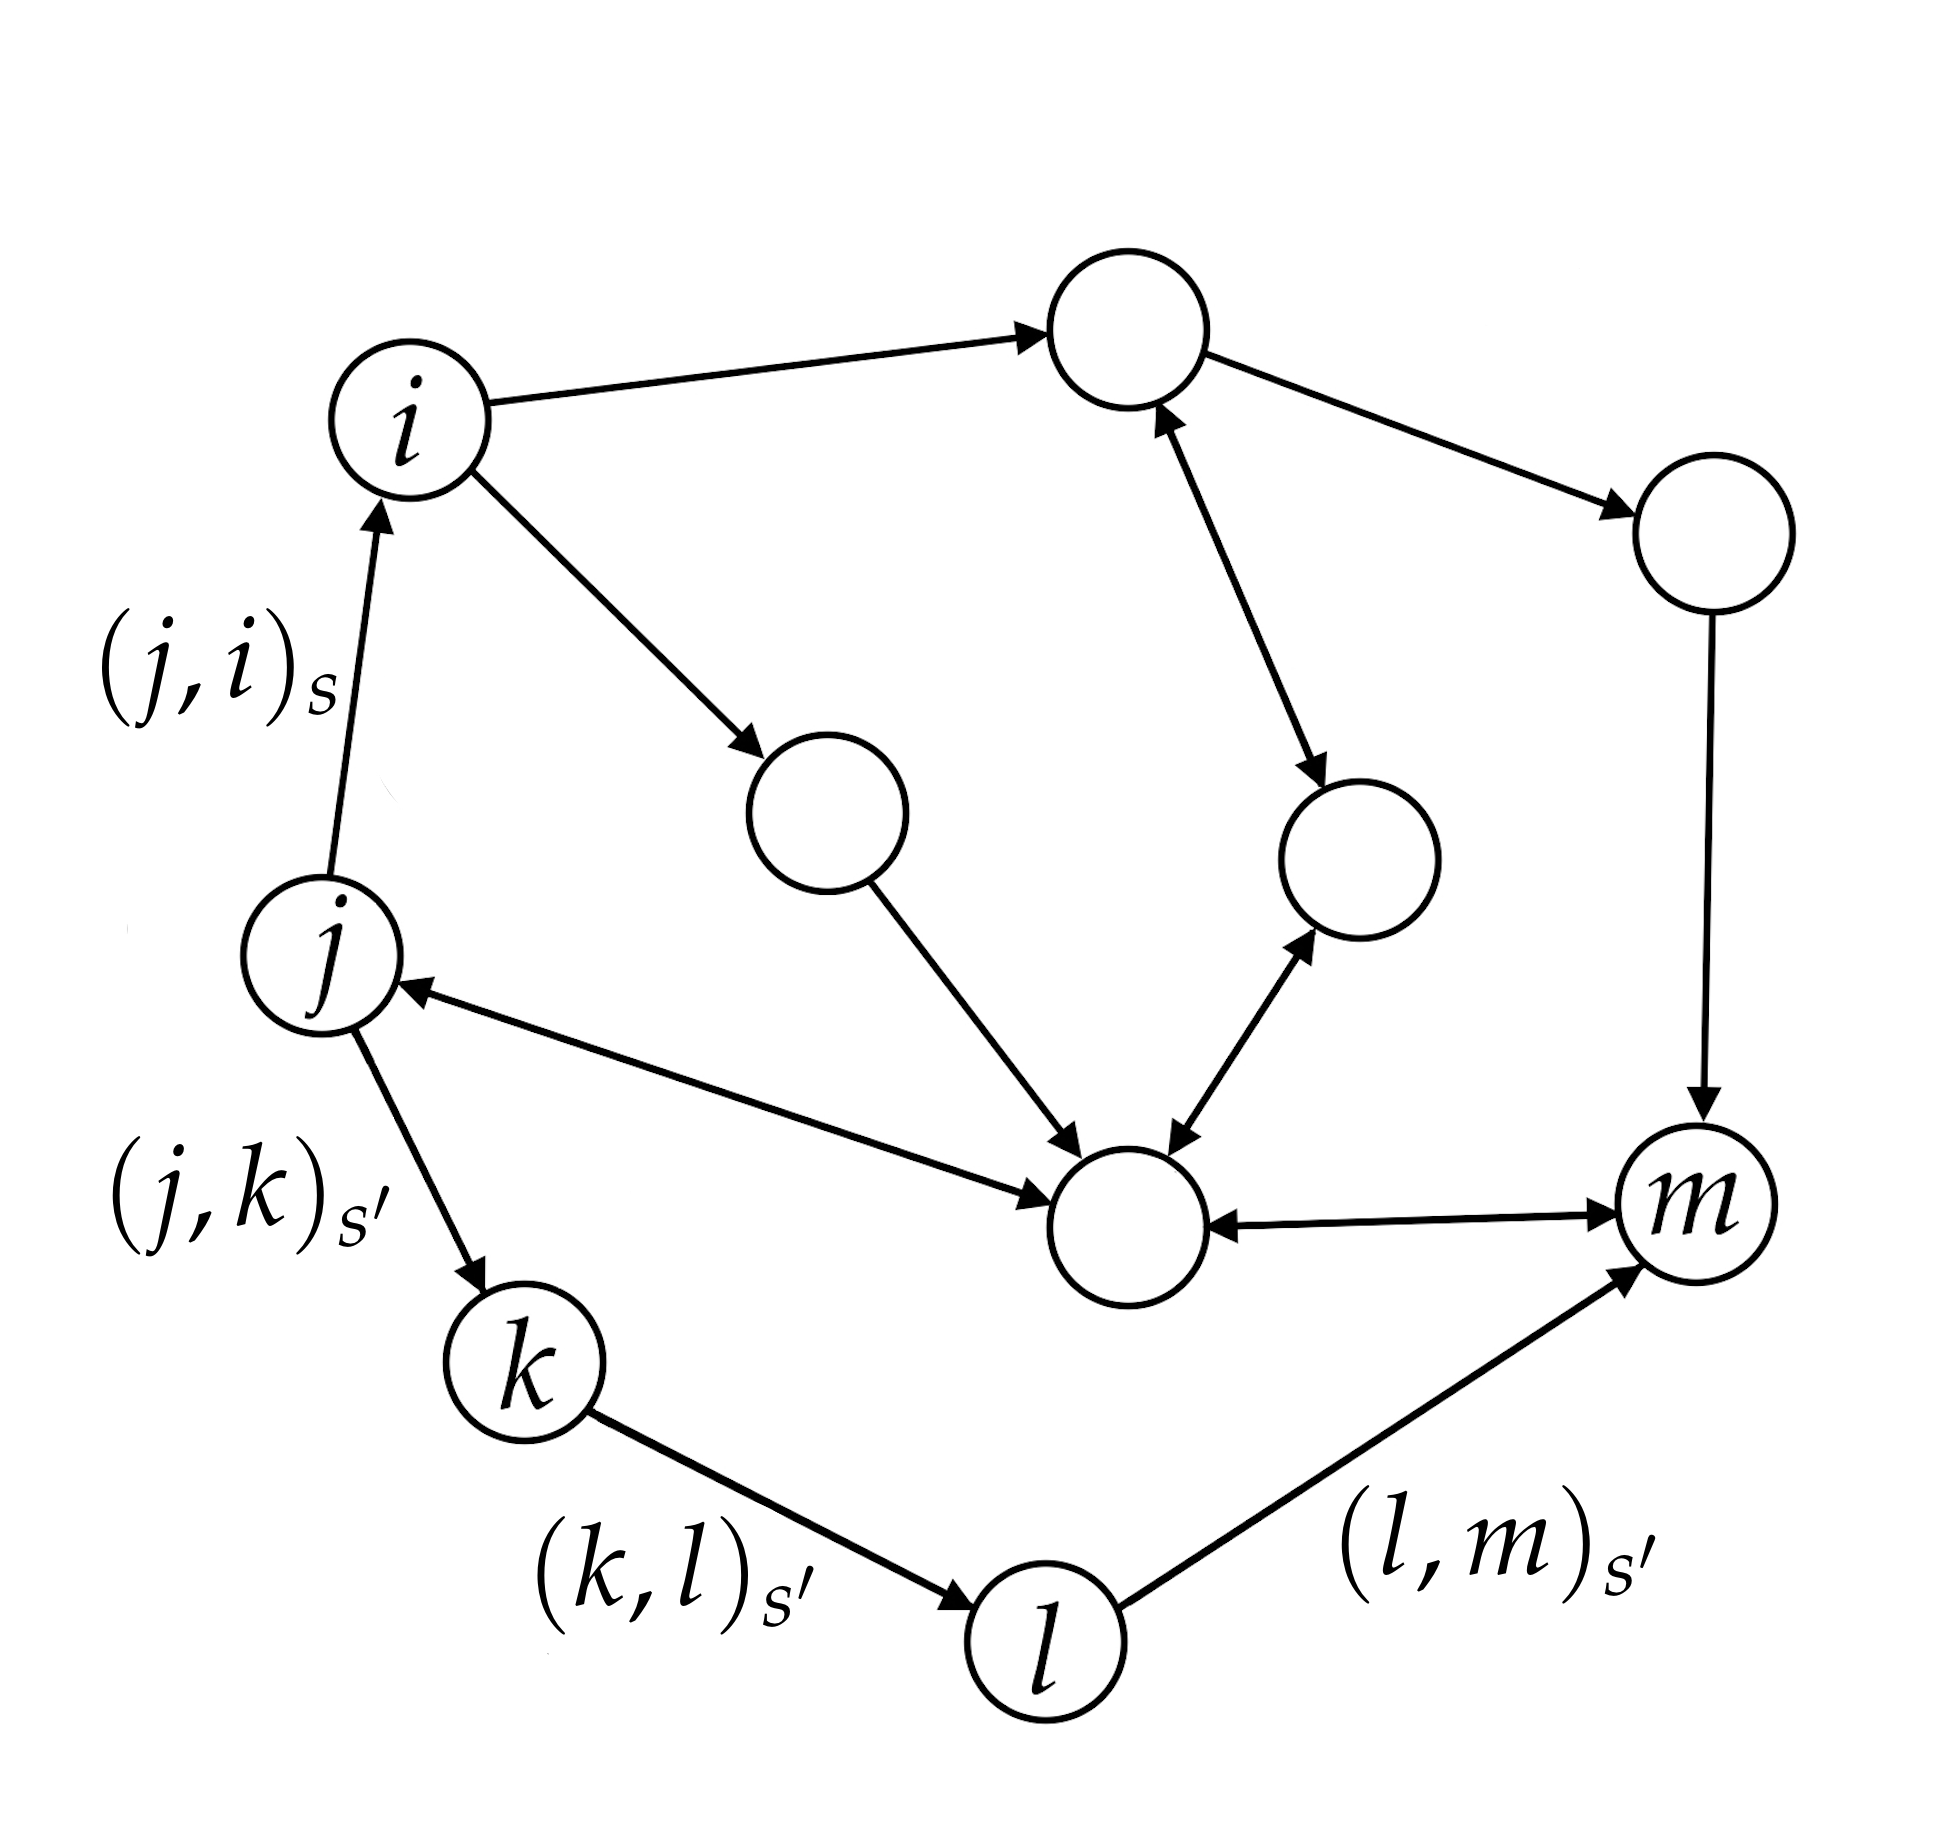
\includegraphics[width=0.7\linewidth]{Figures/Theory/graph_segment.png}\label{fig:theory/graph_seg} }}%
 
 \caption{Illustrations of (a) a standard graph and (b) the extended graph representation.}
 \label{fig:theory/graphs}
\end{figure}


%$i' \quad j' \quad (i',j') \quad (j',i')$

% https://pdfs.semanticscholar.org/6958/4880efd97a02851ba92d4b9d9784996a1055.pdf
% \citep{graphlet_kernels}

%========================================================================%
\section{Extended graph representation}
\label{chp:theory:sec:extgraph}
%========================================================================%

To model the road network a graph will be used. In section \ref{chp:theory.sec:graph} an edge was said to connect two nodes. The graph representation will now be extended to describe the road network in more detail. A segment is a set of consecutive edges or a single edge beginning and ending at an intersection. The intermediate nodes in the segment are connected to two other nodes. Furthermore the head and tail node of the segment (start and end node) are denoted intersection nodes. An intersection node is connected to at least three other nodes. Figure \ref{fig:theory/graph_seg} illustrates this representation. Segment $s$ consists of a single edge $(j,i)$ with head node $j$ and tail node $i$. Segment $s'$ consists of three consecutive edges in order $(j,k), (k,l), (l,m)$ with head node $j$ and tail node $m$. Node $i, j$ and $m$ are intersections. For proper definitions of intersection node, segment, edge and intermediate nodes we refer to table \ref{tab:def}.
% (The intermediate nodes in the segment have degree two. (not if in two directions.))
\iffalse
\begin{figure}[H]
    \centering
    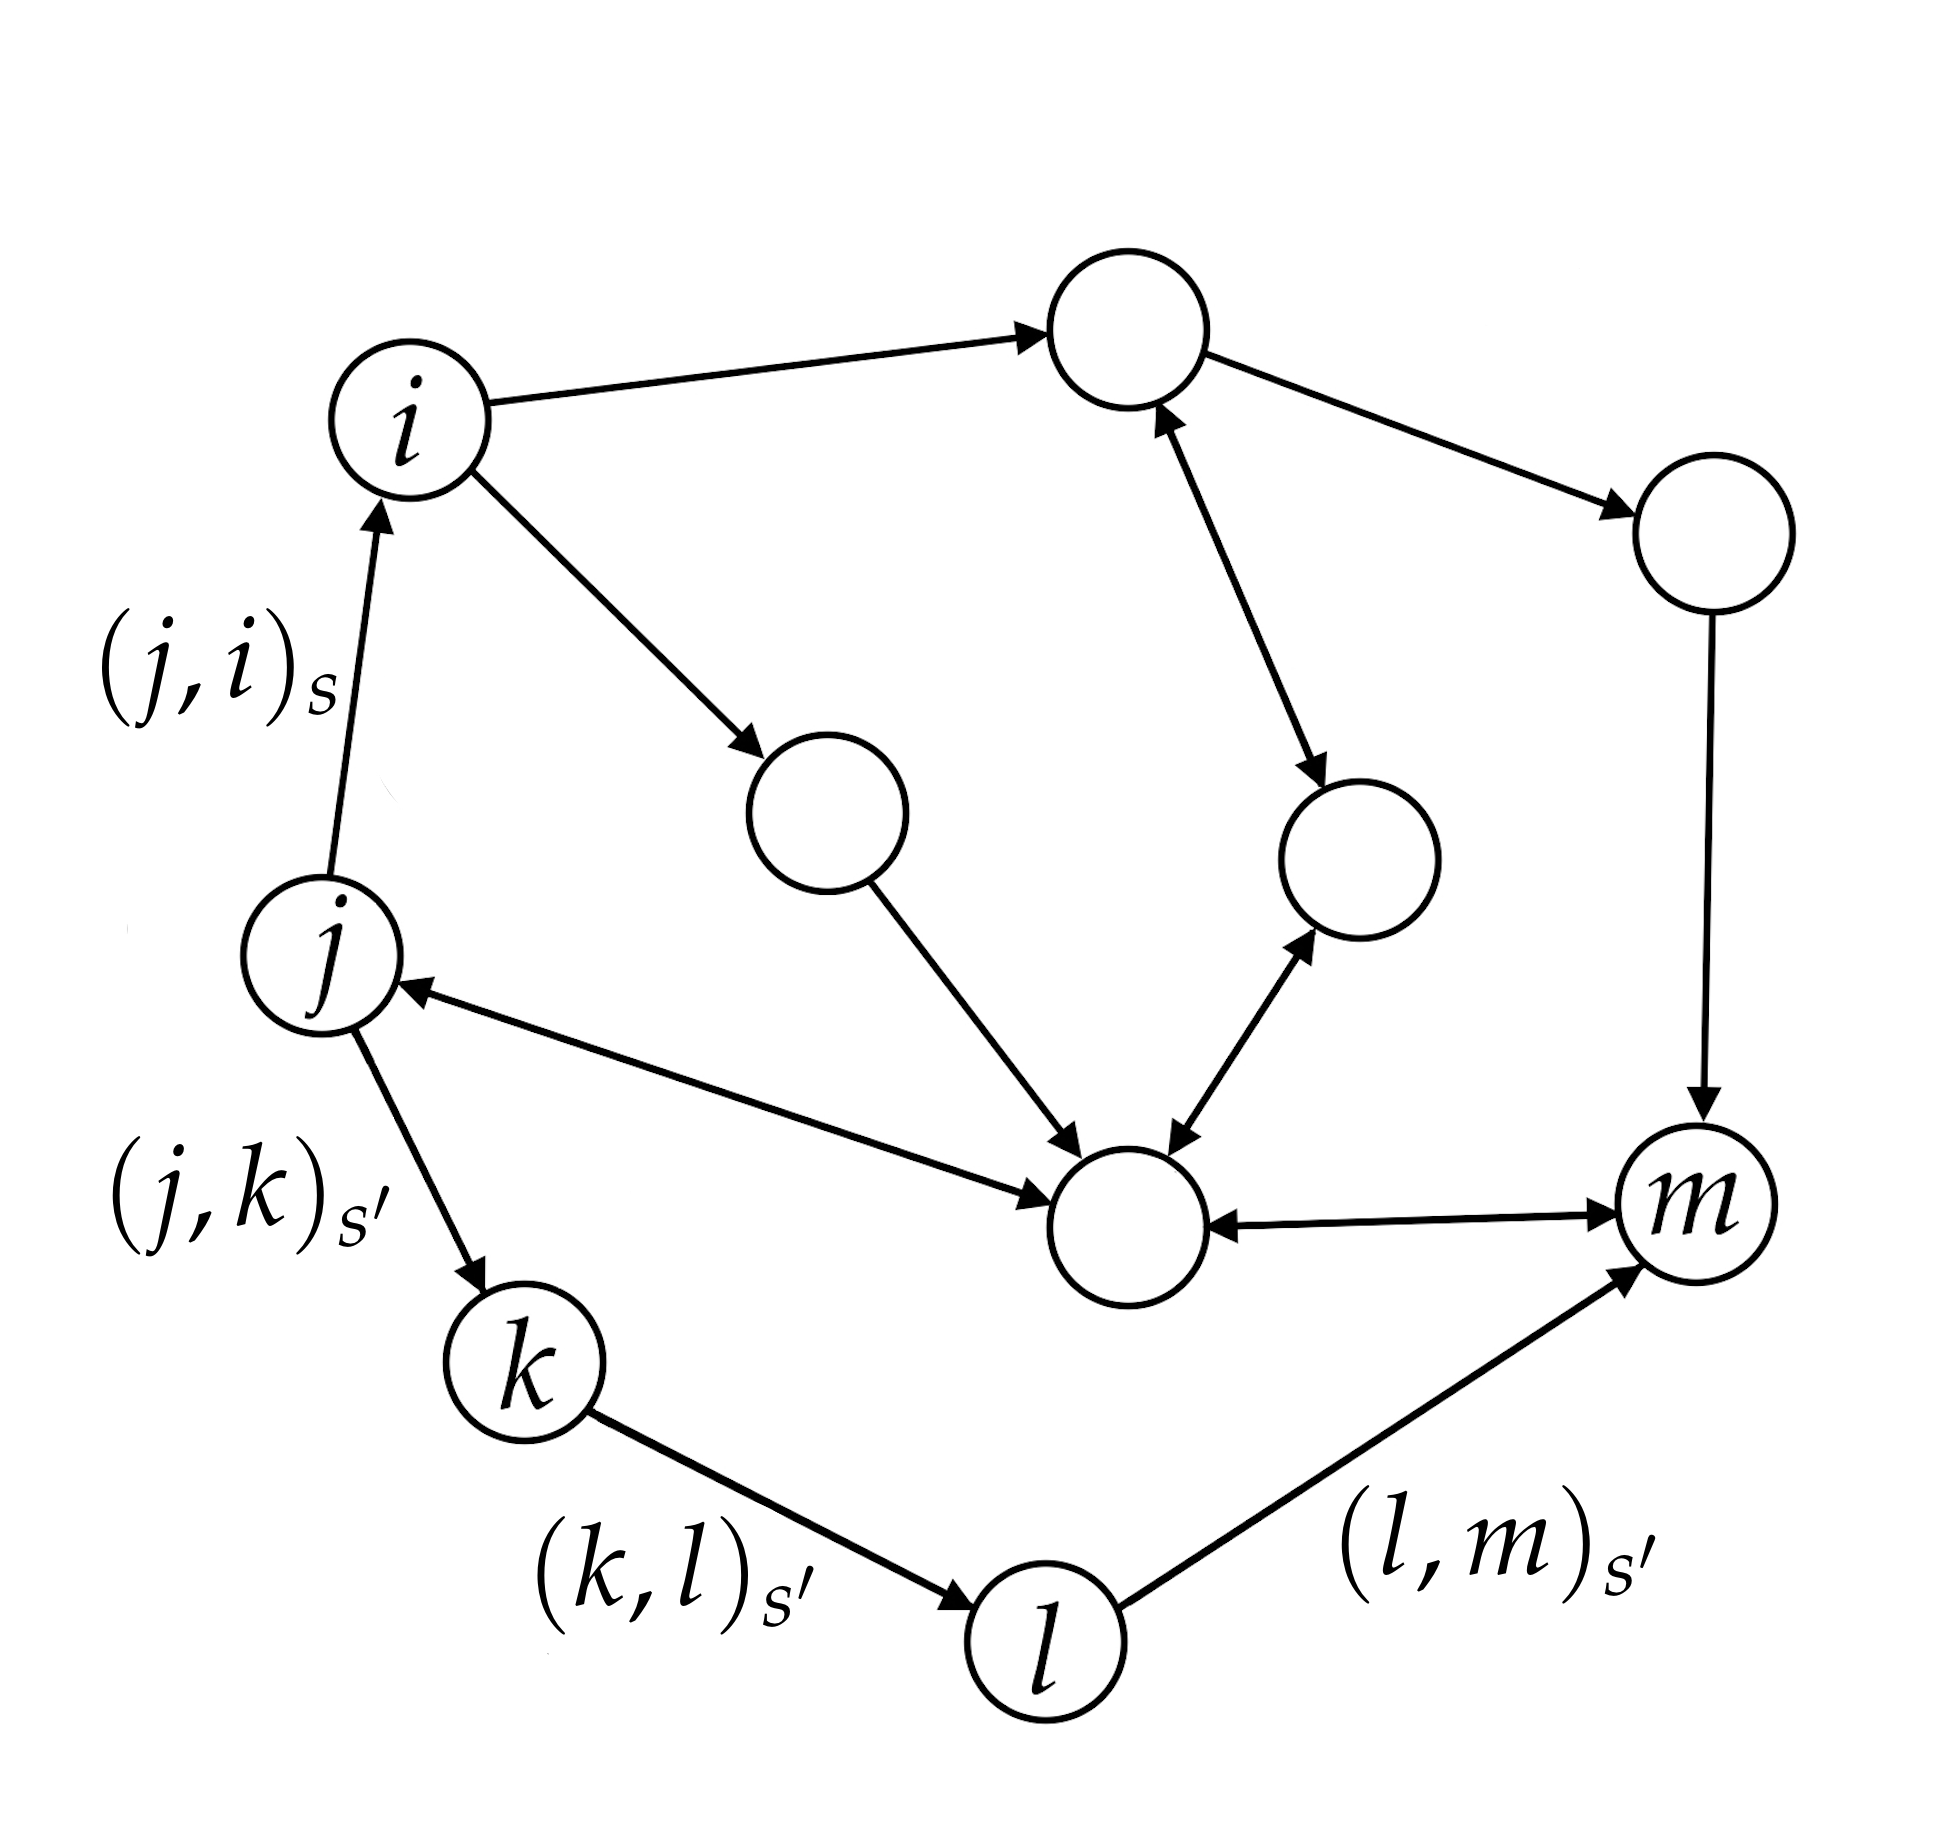
\includegraphics[width=0.6\linewidth]{Figures/Theory/graph_segment.png}
    \caption{Segments and edges using our representation.}
    \label{fig:theory/graph_seg}
\end{figure}
\fi


%========================================================================%
\section{Hidden Markov Model}
\label{chp:theory:sec:HMM}
%========================================================================%

The following section is based on theory from \citep{kondaveeti:clusters}, \citep{HMMstanford}.

An Hidden Markov Model (\ac{HMM}) is a mathematical model and statistical tool for modelling sequential data, assuming it to be a sequence characterised by a Markov process generating an observable sequence. 

%%%%%
% Hidden Markov Model (HMM) is a statistical Markov model in which the system being modeled is assumed to be a Markov process with unobserved (i.e. hidden) states.

% A Hidden Markov Model (HMM) is a statistical tool for modeling generative sequences that can be characterized by an underlying process generating an observable sequence.

% A hidden Markov model (HMM) is a statistical model that can be used to describe the evolution of observable events that depend on internal factors, which are not directly observable

% The Hidden Markov Model (HMM) is a relatively simple way to model sequential data. A hidden Markov model implies that the Markov Model underlying the data is hidden or unknown to you. More specifically, you only know observational data and not information about the states. In other words, there’s a specific type of model that produces the data (a Markov Model) but you don’t know what processes are producing it. You basically use your knowledge of Markov Models to make an educated guess about the model’s structure.
%%%%%

% “One of the applications of HMM, is to predict the sequence of state changes, based on the sequence of observations.”

% He learns that HMM can be used to model a system that 
% 1. Has finite internal states that generate a set of external events (observations)
% 2. The internal state changes are invisible (hidden) to a viewer outside the system
% 3. The current state is always dependent on the immediate previous state only (Markov process)

%%
% A hidden Markov model (HMM) is a statistical model in which the system being modeled is assumed to be a Markov process with unknown parameters.

% stochastic process '= random process
%%%%%

A Markov process is a stochastic process satisfying the Markov property, which states that the transition probability to a successive state is only dependent on the current state. A Markov chain is an instance of a Markov process, defined by a finite set of states and transition probabilities between states in discrete or continuous time. 
It can be seen as a probabilistic graphical model, with edge weights given by the probabilities of each state transition. It can further be time-homogeneous, or stationary, such that the probability of a transition is independent of the point in time at which it occurs in the sequence. 

In an \ac{HMM} the system being modelled is assumed to be a Markov process with unknown parameters such that only observational data is available and no information is available about the states.

% Important classes of stochastic processes are Markov chains and Markov processes. A. Markov chain is a discrete-time process for which the future behaviour, given the past and the present, only depends on the present and not on the past. A Markov process is the continuous-time version of a Markov chain.

Let an \ac{HMM} be defined by a finite state space 

\begin{align}
    S &= \{s_1, s_2, ..., s_N\}
\end{align}

with $N$ hidden or unknown states and let furthermore

\begin{align}
    O &= \{o_1, o_2, ..., o_M\} 
\end{align}

be the observation state space with $M$ observations. 

Further, let $(x_t, y_t)$, $t = (1, 2, ..., T)$, be the Hidden Markov process where $x_t$ is a homogeneous Markov chain, $x_t \in S$, and $y_t$ is the observation sequence, $y_t \in O$. The parameters for the \ac{HMM} are $\theta = (A, B, \pi)$, where the transition probability matrix 

\begin{equation}
    A = [a_{ij}], \quad a_{ij} = P(x_t = s_j | x_{t-1} = s_i), \quad \sum_{j=1}^N a_{ij} = 1 \text{  } \forall i
\end{equation}

consists of transition probabilities $a_{ij}$ from state $s_i$ to state $s_j$ in one step. The emission array 

\begin{equation}
    B = [b_i(o_k)], \quad b_i(o_k) = P(y_t = o_k | x_t = s_i)
\end{equation}

describes the likelihood of being in state $s_i \in S$ and observing $o_k \in O$. Furthermore the initial probability distribution array 

\begin{equation}
    \pi = [\pi_i], \quad \pi_i = P(q_0 = s_i), \quad \sum_{i=1}^N \pi_i = 1 
\end{equation}

describes the likelihood that the Markov chain starts in state $s_i$. Here $q_0$ is the initial state.

Two simplifying assumptions are made when using the first-order \ac{HMM} model. The Markov assumption states that the probability of a certain state only depends on the previous state

\begin{equation}
    P(x_t | x_{t-1}, x_{t-2}, ..., x_1) = P(x_t | x_{t-1}).
\end{equation}

The independence assumption states that the likelihood of an output observation at time $t$ is only dependent on the state that produced the observation. It is independent of all other states and observations

\begin{equation}
    P(y_t | y_{t-1}, y_{t-2}, ..., y_1, x_t, x_{t-1}, ..., x_1) = P(y_t | x_t).
\end{equation}


\cite{Rabiner} proposed that an \ac{HMM} should be defined by the following three central problems:

\newpage
Problem 1: Likelihood\\
Determine the probability $P(y_t | \theta)$ of an observation sequence $y_t \in O$ given a set of parameters $\theta$, defining the \ac{HMM}. 

Problem 2: Decoding\\
Determine the most probable hidden state sequence $x_t \in S$ given an observation sequence $y_t \in O$ and the \ac{HMM} $\theta$. 

Problem 3: Learning\\
Estimate the parameters $\theta$ given an observation sequence $y_t \in O$ and a set of states $S$.



%Model with states and observations. Have emission probability matrix $B$ and transition probability $A$.


%========================================================================%
\section{The Viterbi algorithm} % Decoding
%========================================================================%
The following section is based on theory from \citep{HMMstanford}\citep{viterbi}.


The Viterbi algorithm, a kind of dynamic programming, is the most common decoding algorithm for \ac{HMM}s. It is an algorithm solving ``Problem 2: Decoding'' in section \ref{chp:theory:sec:HMM}.



The basic idea is to process the observation sequence from the last observation to the first, maximising over the likelihood of all possible paths leading to our current state. More formally, given an \ac{HMM} $\theta = (A, B, \pi)$ and a sequence of observations $Y = [y_t]$, $y_t \in O$, each cell in the dynamic programming table is given by

\begin{equation}
    v_t(j) = \max_{x_1,\ldots,x_{t-1}} P(x_1,\ldots,x_{t-1}, y_1, y_2, \ldots, y_t, x_t = s_j | \theta)
\end{equation}

where $v_t(j)$ denotes the Viterbi probability for the cell and the maximisation over all possible previous states $\max_{x_1, \ldots, x_{t-1}}$ gives the most probable path up to time $t$. We compute these probabilities recursively as the product of the Viterbi probability in the previous time step, the transition probability $a_{ij}$ from possible previous states $s_i$ and the emission probability $b_j(o_t)$

\begin{equation}
    v_t(j) = \max_{1\leq i\leq N} v_{t-1}(i)a_{ij}b_j(o_t).
\end{equation}

Once the most probable path has been computed, where in each step the Viterbi probability is maximised, a back tracing step is performed to obtain the most probable sequence of states. The computational complexity of the Viterbi algorithm is proportional to the number of observations and hidden states, in the order $O(TN^2)$. The pseudo code for the Viterbi algorithm is found below in algorithm \ref{alg:viterbi}.

\begin{algorithm}[H]
    \caption{Viterbi}
    \label{alg:viterbi}
    \begin{algorithmic}
    \Function{Viterbi}{observations $Y$, state space $S$, model $\theta = (A, B, \pi)$} 
    
    
    \For{state $s_j \in S$ \textbf{from} $1$ \textbf{to} $N$}
    %\State $v[j,1] \gets a_{q_0,j}b_j(o_1)$ \Comment{initialisation step}
    \State $v[j,1] \gets \pi_j b_j(o_1)$
    \State $backtrace[j,1] \gets 0$ \Comment{initialisation step}
    \EndFor
    
    \For{time step $t$ \textbf{from} $1$ \textbf{to} $T$} % time step $t = 1, \ldots, T$ ?
    \For{state $s_j \in S$ \textbf{from} $1$ \textbf{to} $N$}
        \State $v[j,t] \gets \max_{s_i \in S}v[i,t-1]a_{i,j}b_j(o_t)$ 
        \State $backtrace[j,t] \gets\text{argmax}_{s_i\in S} v[i, t-1]a_{i,j}$
    \EndFor
    \EndFor
    
    %\State $v[x_T, T] \gets \max_{s_i \in S}v[i, T]a_{i,x_T}$ \Comment{termination step}
    %\State $backtrace[x_T, T] \gets \text{argmax}_{s_i\in S}v[i, T]a_{i,x_T}$ \Comment{termination step}
    
    \State $x_T = \text{argmax}_{s_j \in S} v[j,T]$
    
\State \textbf{return} most probable path from $backtrace[x_T, T]$
\EndFunction
\end{algorithmic}
\end{algorithm}

%https://en.wikipedia.org/wiki/Viterbi_algorithm#Pseudocode

%========================================================================%
\section{Map generation}
%========================================================================%

%------------------------------------------------------------------------%
\subsection{Kernel Density Estimation}
%------------------------------------------------------------------------%
\label{chp:theory.sec:kde}

A common technique in statistics to estimate the probability density function of a random variable given a finite number of samples is to do a \ac{KDE} \citep{terrell1992}.

However, an approximate \ac{KDE} will be used according to the following methodology \citep{4inBiagioni}. Initially the area of interest is discretised into a grid with desired cell size. For this application an appropriate cell size is one that is a fraction of the road width. Then a 2D histogram is created by computing the number of times each trajectory or point, see table \ref{tab:def}, in the data set passes a cell. This 2D histogram is furthermore smoothed by convolving it with a two-dimensional Gaussian kernel

\begin{equation}\label{eq:gaussian}
    G(x,y;\sigma) = \frac{1}{2\pi \sigma^2} e^{-((x^2+y^2)/2\sigma^2)}    
\end{equation}

\citep{bookImageAnalysis}. This methodology fast produces a good approximate \ac{KDE} \citep{biagioni:gis12}. It is an approximation due to the cells in the grid. The accuracy of this approximation is inversely proportional to the size of the grid cells.

%------------------------------------------------------------------------%
\subsection{Skeletonization} 
\label{chp:theory.sec:mapgen.sub:skeleton}
%------------------------------------------------------------------------%

Skeletonization is a method for extracting the skeleton of a binary image by removing all contour points except those belonging to the skeleton, by applying a thinning algorithm to the image. \cite{Zhang:skeleton} suggests appropriate rules to follow when performing a skeletonization. 
The procedure is iterative and performed for every iteration pixel $P_1$ in figure \ref{tab:theory/8neigh}. Let $A(P_1)$ be the number of $(0, \geq 1)$-pairs in the 8-neighbourhood of $P_1$ ordered as $(P_2, P_3), (P_3, P_4), \ldots, (P_8, P_9), (P_9, P_2)$. Let $B(P_1)$ be the total number of non-zero pixels in the neighbourhood. Each iteration pixel $P_1$ in figure \ref{tab:theory/8neigh} is deleted if it satisfies the following conditions:

\begin{align}
   A(P_1) = 1 \\
   2 \leq B(P_1) \leq 6 \\
   P_2\cdot P_4\cdot P_6 \neq 1 \label{c} \\ 
   P_4\cdot P_6\cdot P_8 \neq 1 \label{d}.
\end{align}

% The procedure is iterative and each iteration pixel $P_1$ in figure \ref{tab:theory/8neigh} is deleted if it satisfies the following conditions:
% $A(P_1)$ is the number of $(0, \geq 1)$-pairs in the 8-neighbourhood of $P_1$ 
In a second subiteration conditions (\ref{c}) and (\ref{d}) are changed to 

\begin{align}
    P_2\cdot P_4\cdot P_8 = 1 \\ 
   P_2\cdot P_6\cdot P_8 = 1 
\end{align}

Finally, any pixel satisfying $B(P_1) \geq 7$ is set to zero.



\begin{figure}[H]
\centering
\begin{tabular}{|c|c|c|}
\hline
$P_9$ & $P_2$ & $P_3$ \\
$(i-1, j-1)$ & $(i-1, j)$ & $(i-1, j+1)$ \\ \hline
$P_8$ & $P_1$ & $P_4$ \\
$(i, j-1)$ & $(i, j)$ & $(i, j+1)$ \\ \hline
$P_7$ & $P_6$ & $P_5$ \\
$(i+1, j-1)$ & $(i+1, j)$ & $(i+1, j+1)$ \\ \hline
\end{tabular}\caption{8-neighbourhood of pixel $P_1$. $(i,j)$ give the pixel indices in the image.}
\label{tab:theory/8neigh}
\end{figure}

%\vspace{1.15cm}



% skeletonization
% graph
% f-score evaluation
% kde

%------------------------------------------------------------------------%
\subsection{Combustion algorithm}
\label{chp:theory.sec:mapgen.sub:comb}
%------------------------------------------------------------------------%

\textbf{NOT FINISHED}

Given a binary skeleton of a road network, where road pixels are given by 1 and empty pixels by 0, we would like to extract a graph representation of roads and intersections with structure defined in section \ref{chp:theory:sec:extgraph}. One way of doing this is presented by \cite{21inBiagioni}. Intersection nodes are first found by studying the neighbourhood of each pixel and then applying a combustion algorithm to find paths between them.

Define the 24-neighbourhood of pixel $P_1$ as in figure \ref{tab:theory/comb}. Further, define a connected component as a sequence of two pixels connecting pixel $P_1$ to the edge of its $5\times 5$-neighbourhood, i.e. a two step 8-connected sequence. To detect crossing pixels, future intersection nodes, the idea is to iterate through all road pixels in the image and for each pixel count the number of connected components. If this value is larger than 2 or equal to 1, representing a dead end, the pixel is marked as a crossing, represented by the value 2. 

An illustration of such components can be seen in figure \ref{fig:theory/conncomp}, where each box corresponds to a pixel in figure \ref{tab:theory/comb}. A black box corresponds to pixel value 1 and a white to 0. We here illustrate the possible configurations once, the remaining cases can be found symmetrically by mirroring and rotation. 

For each outer pixel, we count the connected component if at least one connecting sequence can be found, i.e. if at least one of the configurations in figure \ref{fig:theory/conn1}, \ref{fig:theory/conn2} and \ref{fig:theory/conn3} respectively can be found.  

\textbf{List of rules!!!!!!}

\begin{figure}[H]
\centering
\begin{tabular}{|c|c|c|c|c|}
\hline
$P_{24}$ & $P_{25}$ & $P_{10}$ & $P_{11}$ & $P_{12}$ \\
(i-2,j-2) & (i-2,j-1) & (i-2,j)   & (i-2,j+1) & (i-2,j+2) \\ \hline
$P_{23}$ & $P_{9}$  & $P_{2}$  & $P_{3}$  & $P_{13}$ \\
(i-1,j-2) & (i-1,j-1) & (i-1,j)   & (i-1,j+1) & (i-1,j+2) \\ \hline
$P_{22}$ & $P_{8}$  & $P_{1}$  & $P_{4}$  & $P_{14}$ \\
(i,j-2)   & (i,j-1)   & (i,j)     & (i,j+1)   & (i,j+2)  \\ \hline
$P_{21}$ & $P_{7}$  & $P_{6}$  & $P_{5}$  & $P_{15}$ \\
(i+1,j-2) & (i+1,j-1) & (i+1,j)   & (i+1,j+1) & (i+1,j+2) \\ \hline
$P_{20}$ & $P_{19}$ & $P_{18}$ & $P_{17}$ & $P_{16}$ \\
(i+2,j-2) & (i+2,j-1) & (i+2,j)   & (i+2,j+1) & (i+2,j+2) \\ \hline
\end{tabular}
\caption{24-neighbourhood of pixel $P_1$. $(i,j)$ gives the pixel indices in the image.}
\label{tab:theory/comb}
\end{figure}


\begin{figure}[H]%
 \centering
 \subfloat[\textit{Case 1.}]{{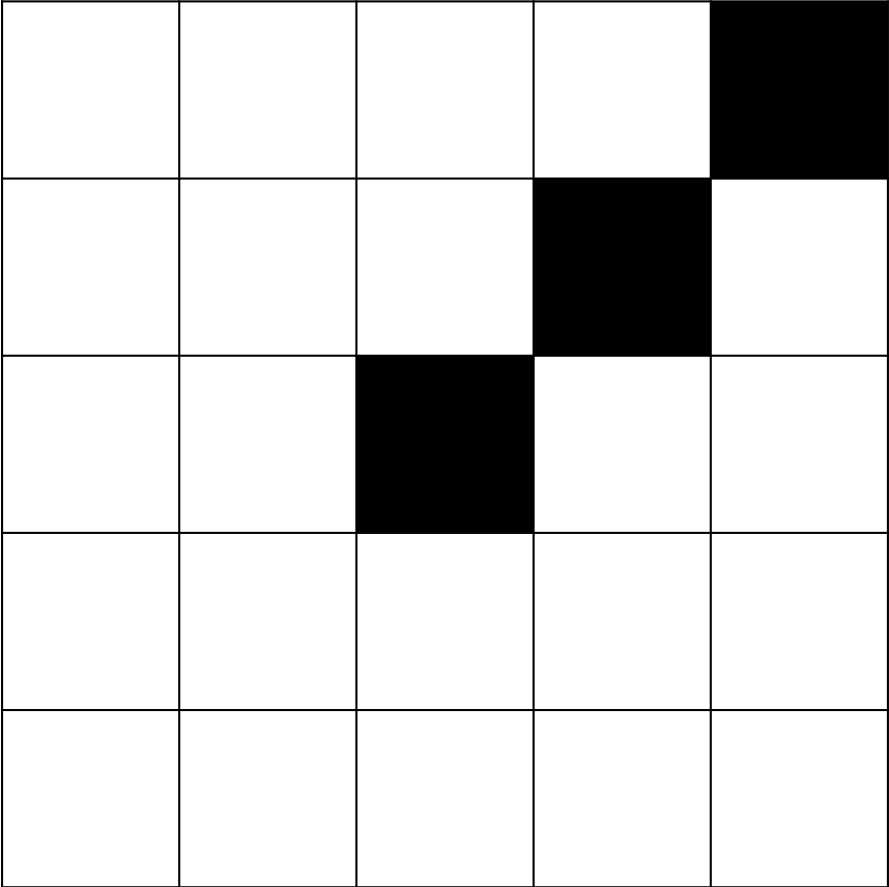
\includegraphics[height=0.17\linewidth]{Figures/Theory/conn1.png}\label{fig:theory/conn1} }}% 
 \quad \quad \quad
 \subfloat[\textit{Case 2.}]{{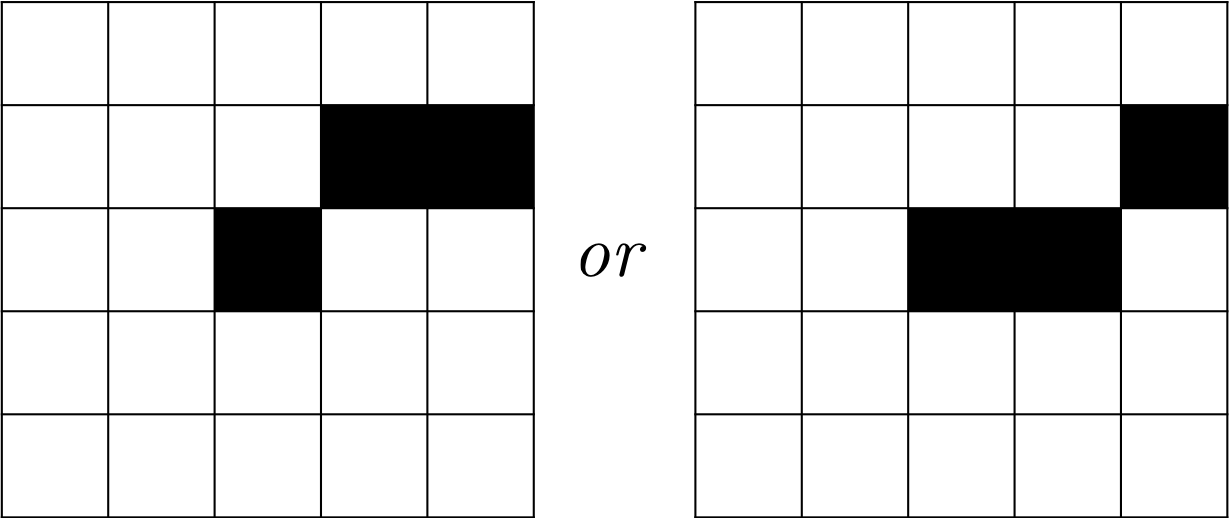
\includegraphics[height=0.17\linewidth]{Figures/Theory/conncomp1.png}\label{fig:theory/conn2} }}%
 \vspace{1.5em}
 \subfloat[\textit{Case 3.}]{{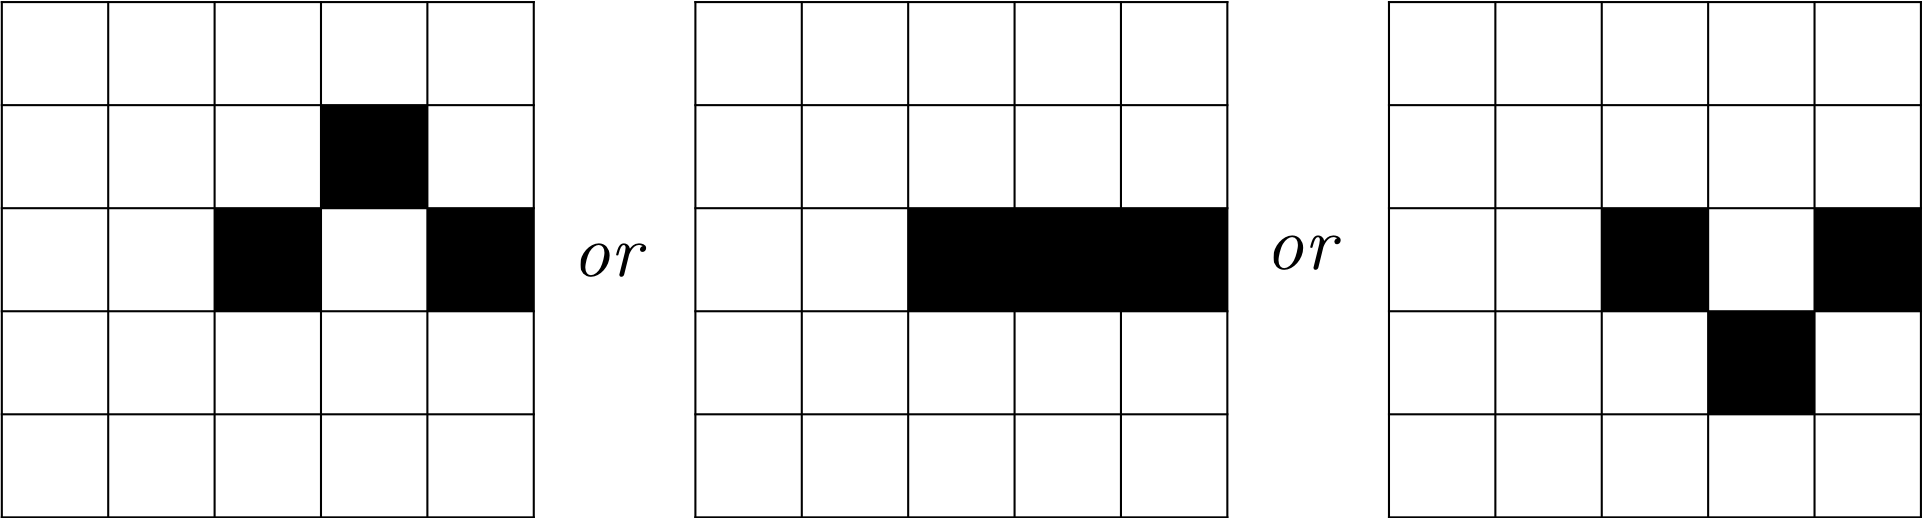
\includegraphics[height=0.17\linewidth]{Figures/Theory/conncomp2.png}\label{fig:theory/conn3} }}%
 \caption{The possible 8-connected components used to define intersections. The remaining cases can be found symmetrically. Each cell corresponds to a pixel in the 24-neighbourhood of the central pixel.}%
 \label{fig:theory/conncomp}
\end{figure}

To extract the sequence of pixels, road segments, connecting each intersection, an extended combustion algorithm is performed. For each crossing pixel the neighbouring pixels are checked, in each direction. If the value is 1, the pixel is added to a list of segment pixels. Once a crossing pixel has been found the value is set to 3 to flag it as visited. The pseudo code can be seen in algorithm \ref{alg:comb}.

\begin{algorithm}[H]
    \caption{Extended Combustion}
    \label{alg:comb}
    \begin{algorithmic}
    
    \State clear stack \textit{crossing}
    \State $p(i,j) \gets 3$
    \State push $(i,j)$ into queue \textit{combusting}
    \While{\textit{combusting} $\neq$ \{\}}
        \State $(m,n) \gets$ \textit{combusting}'s head element
        \State pop \textit{combusting}'s head element
        \State push $(m,n)$ into stack \textit{crossing}
        \For{\textbf{all} $p(i,j)$'s neighbouring pixels}
            \If{the pixel = 2}
                \State the pixel $\gets 3$
                \State push the pixel's coordinates into queue \textit{combusting}
            \EndIf
        \EndFor
    \EndWhile
    \end{algorithmic}
\end{algorithm}

%------------------------------------------------------------------------%
\subsection{Ramer-Douglas-Peucker algorithm}
\label{chp:theory.sec:dp}
%------------------------------------------------------------------------%

% The goal of the Douglas Peucker (DP) algorithm is to reduce the number of points needed to represent a curve while keeping the new curve similar to the original \cite{dp}.
The goal of the \ac{DP} algorithm is to recursively reduce the number of points needed to represent a curve while preserving the curvature \citep{dp}. Define two curves, the original curve and the new curve having been simplified by removal of some points but still having the same curvature. The similarity between the original and new curve is measured by the maximum distance between the curves. More formally, given a curve with $n$ points $X = [p_0, \ldots, p_n]$ we define $\overline{p_0p_n}$ as the line going from point $p_0$ to point $p_n$. For each step in the \ac{DP} recursion we consider the intermediate point $p_i$ giving the maximum perpendicular distance to line $\overline{p_0p_n}$, i.e. the Hausdorff distance. A more formal definition of the Hausdorff distance is given in section \ref{chp:theory.sec:evaluation.sub:stat.sub:dist}. If this distance is greater than a distance $\epsilon$, the curve $X_{0,\ldots,i} = [p_0, \ldots, p_i]$ going from $p_0$ to $p_i$ is recursively simplified as well as $X_{i,\ldots, n} = [p_i, \ldots, p_n]$, until no more simplifications can be done. The pseudocode can be seen in algorithm \ref{alg:dp}.
\begin{algorithm}[H]
    \caption{Douglas Peucker}
    \label{alg:dp}
    \begin{algorithmic}
        \Function{DouglasPeucker}{points vector $X$ of length $n$,  distance $\epsilon$}

    \State $d_{max}, p_i \gets \textsc{HausdorffDistance}(\overline{p_0p_n}, X)$ \Comment{\textit{max distance between curves}}
    \If{$d_{max} > \epsilon$}
        \State $res_{p_0p_i} \gets \textsc{DouglasPeucker}(X_{0,\ldots,i}, \epsilon)$ 
        \State $res_{p_ip_{n}} \gets \textsc{DouglasPeucker}(X_{i,\ldots, n}, \epsilon)$
        \State $res \gets [res_{p_0p_i}, res_{p_ip_{n}}]$
    \Else
        \State $res \gets [p_0, p_n]$
    \EndIf
    
\State \textbf{return} simplified vector $res$
\EndFunction
    \end{algorithmic}
\end{algorithm}


%========================================================================%
\section{Evaluation}
%========================================================================%

In this section we present the evaluation statistics, both statistical metrics and distance measures, that will be used to evaluate the generated maps. Furthermore, three methodologies for evaluating graphs representing road networks are presented.

%------------------------------------------------------------------------%
\subsection{Evaluation statistics}
%------------------------------------------------------------------------%
\label{chp:theory.sec:evaluation.sec:stat}

%........................................................................%
\subsubsection{F-score}
\label{chp:theory.sec:evaluation.sub:stat.sub:fscore}
%........................................................................%

In binary classification tasks precision is defined as the number of true positives ($tp$) divided by the total number of elements labelled as belonging to the positive class. The denominator is given by the sum of true positives and false positives ($fp$), the number of elements falsely labelled as belonging to the class. We denote precision as

\begin{equation}
    precision = \frac{tp}{tp + fp}.
\end{equation}

Recall is defined as the number of true positives ($tp$) divided by the total number of elements that actually belong to the positive class. The denominator is given by the sum of true positives and false negatives ($fn$), the object is falsely classified as not belonging to the class. We denote recall as

\begin{equation}
    recall = \frac{tp}{tp + fn}.
\end{equation}

An illustration can be seen in figure \ref{fig:theory/precrec}. The F-score 

\begin{equation} \label{eq:fscore}
    F\text{-}score = 2\cdot\frac{precision\cdot recall}{precision + recall}
\end{equation}

is given by the harmonic mean of precision and recall \citep{precisionrecall}. This means it will only give a high score if both precision and recall are high.

\begin{figure}[H]
    \centering
    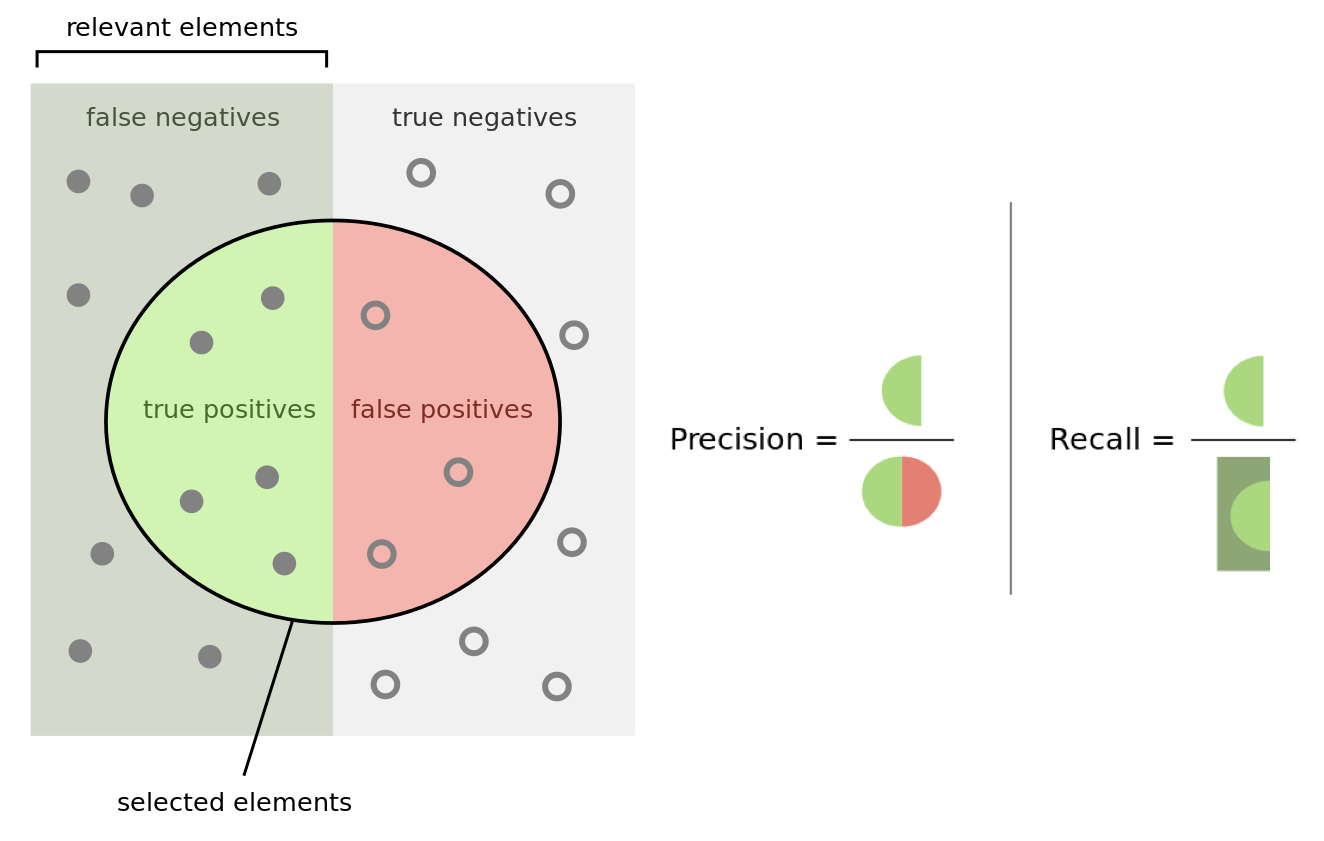
\includegraphics[width=13cm]{Figures/Theory/Precisionrecall.png}
    \caption{Illustration of precision and recall, inspired by \citep{wiki:prerecall}.}
    \label{fig:theory/precrec}
\end{figure}

%........................................................................%
\subsubsection{Distance measures}
\label{chp:theory.sec:evaluation.sub:stat.sub:dist}
%........................................................................%


\textbf{Hausdorff distance}

There exists several distance measures for polylines. Let $d$ denote the underlying distance metric in the plane, for example the Euclidian distance. One common measure is known as the \textit{Hausdorff distance}. We define two \textit{directed Hausdorff distances} for bounded point sets $A, B \subseteq \mathbb{R}^2$ as

\begin{equation}
\begin{split}
    \label{eq:dhausdorff}
    \overrightarrow{\delta_H}(A,B) = \sup_{a\in A} \inf_{b\in B} d(a, b) \\
    \overrightarrow{\delta_H}(B,A) = \sup_{b\in B} \inf_{a\in A} d(b, a)
\end{split}
\end{equation}

and one \textit{undirected Hausdorff distance} defined for bounded point sets $A, B \subseteq \mathbb{R}^2$ as

\begin{equation}
\label{eq:udhausdorff}
    \delta_H(A,B) = \max(\overrightarrow{\delta_H}(A,B), \overrightarrow{\delta_H}(B,A)).
\end{equation}

Let two polylines be represented by two point sets $A$ and $B$. We first calculate all distances between a point $a \in A$ in one set and its closest point $b \in B$ in the other set. By taking the maximum over all these minimum distances we obtain the \textit{Hausdorff distance} between the two polylines. This distance measure captures the worst case behaviour, and is not a linear distance metric \citep{distances}.

%is thus obtained by taking the maximum over all minimum distances between a point and its closest point in the other set in the two sets representing the lines. 

\newpage
\textbf{Fréchet distance}

Another common distance measure for polylines is the \textit{Fréchet distance}, defined for planar curves $f, g : [0,1] \rightarrow \mathbb{R}^2$ as

\begin{equation}
\label{eq:frechet}
    \delta_F(f,g) = \inf_{\alpha}\max_{t\in [0,1]} d(f(t), g(\alpha(t))) 
\end{equation}

for continuous, monotone increasing one-to-one mappings $\alpha$ \citep{distances}.

The Fréchet distance is a measure of similarity between two curves, $f$ and $g$. Imagine a man and a dog walking on one curve each with a leash in between. The Fréchet distance is defined as the minimum leash length sufficient to join the two travelling forward along the two curves, although the rate of travel for either of them may not necessarily be uniform. The parameter $t$ can here be thought of as ``time''. At time $t$, the length of the leash is given by the distance between $f(t)$ and $g(\alpha(t))$. Taking the infimum over all possible reparametrisations $\alpha$ corresponds to the walk where the maximum leash length is minimised.

\iffalse
Informally, we can think of the parameter {\displaystyle t} t as ``time''. Then, {\displaystyle A(\alpha (t))} A(\alpha (t)) is the position of the dog and {\displaystyle B(\beta (t))} B(\beta (t)) is the position of the dog's owner at time {\displaystyle t} t (or vice versa). The length of the leash between them at time {\displaystyle t} t is the distance between {\displaystyle A(\alpha (t))} A(\alpha (t)) and {\displaystyle B(\beta (t))} B(\beta (t)). Taking the infimum over all possible reparametrizations of {\displaystyle [0,1]} [0,1] corresponds to choosing the walk along the given paths where the maximum leash length is minimized. The restriction that {\displaystyle \alpha } \alpha  and {\displaystyle \beta } \beta  be non-decreasing means that neither the dog nor its owner can backtrack.
\fi

Unlike the Hausdorff distance, the Fréchet distance takes continuity and monotonicity of the curves into account, making it more suitable for comparing, for example, paths in a graph \citep{pathbased}.

%Further, the Hausdorff distance allows for graphs with very different topology to be classified as similar \citep{rncomp}. Roads can be very similar geometrically but a travel path within one graph can be connected while the other one is disconnected (see fig 1).

\textbf{Great-circle distance}

To compute the great-circle distance, $d_{GC}$, between two points given in longitude and latitude on a sphere the Haversine formula can be used. Considering the sphere to be the earth this calculation will be an approximation, since the earth is not perfectly spherical. 

Let $\theta$ be the central angle between the two points $p_1 = (lon_1, lat_1)$ and $p_2 = (lon_2, lat_2)$ on the sphere, where longitude and latitude are given in radians. The central angle is given as the great circle distance $d_{GC}$ between the points divided by the radius $R$, $\theta = d_{GC} / R$. Further, define the Haversine function as

\begin{equation}
    \text{hav}(\theta) = \sin^2 \left( \frac{\theta}{2} \right)
\end{equation}

The Haversine formula is then defined as

\begin{equation}
    \text{hav}\left( \frac{d_{GC}}{R} \right) = \text{hav}\left(lat_2 - lat_1\right) + \cos\left(lat_1\right) \cos\left(lat_2\right) \text{hav}\left(lon_2 - lon_1\right)
\end{equation}

Solving for $d_{GC}$ gives the great circle distance \citep{haversine}.

%------------------------------------------------------------------------%
\subsection{Evaluation methodology}
\label{chp:theory.sec:evaluation.sec:meth}
%------------------------------------------------------------------------%

The goal of map comparison is to obtain a measure of similarity between maps, or more specifically, graphs. The task of comparing two graphs is well studied \citep{graphlet_kernels} \citep{subgraphmatching} \citep{shortestpath}. Sub graph isomorphism is the amount of change needed to convert one graph exactly into the second graph. Given two graphs G and H, to determine if there exists a sub graph of G which is isomorphic to H has been shown to be NP-complete. It requires comparison of all possible sub graphs, which quickly becomes unfeasible for large graphs \citep{graphlet_kernels}. Sub graph isomorphism is however closely related to what we want to achieve when comparing road network graphs.

According to \cite{graphlet_kernels}, common graph comparison algorithms can be split into three main categories: 
\begin{itemize}
    \item set based
    \item frequent sub graph based
    \item kernel based.
\end{itemize}
Frequent sub graph based methods aim to find reoccurring sub graph structures across several graphs \citep{subgraphmatching}. This method is mostly used in the area of data mining \citep{subsurvey}.

A graph kernel is a kernel function that computes an inner product on graphs. Among kernel based methods, random walk kernels count the number of matching walks in two graphs. This approach will for large graphs become increasingly computationally expensive. Further, random walks allow for repetitions of nodes. This can lead to too high similarity measures, a problem known as \textit{tottering} \citep{shortestpath}. \cite{shortestpath} define a kernel by computing the shortest path distance between all pairs of nodes in the graphs. The shortest path problem can be solved using Dijkstra's algorithm. This computation is cheaper than the random walk, and avoids tottering. 

These types of graph comparison algorithms do not take the spatial orientation of nodes and edges into account, only topological similarities. However, to be able to compare street networks we need to include information also on the geometry of the roads. One type of comparison to include spatial orientation is set based comparisons.













\iffalse
%........................................................................%
\subsubsection{Road network comparison}
%........................................................................%

%........................................................................%
\subsubsection{Graph comparison}
%........................................................................%

Two graphs are said to be isomorphic if they share the same node set, except for relabelling, and share the same connectivity. More formally, two graphs $\mathcal{G}^{(i)} = (\mathcal{V}^{(i)}, \mathcal{E}^{(i)}, W^{(i)})$ for $i=1,2$ are isomorphic if there is a bijection between the node sets of the graphs $f : \mathcal{V}^{(1)} \rightarrow \mathcal{V}^{(2)}$ such that $(i,j) \in \mathcal{E}^{(1)}$ iff $(f(i), f(j)) \in \mathcal{E}^{(2)}$ and $W^{(1)}_{ij} = W^{(2)}_{f(i)f(j)} \forall i,j \in \mathcal{V}^{(1)}$ \citep{giacomo}.

Given two graphs G and H, to determine if there exists a sub-graph of G which is isomorphic to H has been shown to be NP-complete. It requires comparison of all possible sub-graphs, which quickly becomes unfeasible for large graphs \citep{graphlet_kernels}. Sub-graph isomorphism is however closely related to what we want to achieve when comparing road network graphs.

According to \cite{graphlet_kernels}, common graph comparison algorithms can be split into three main categories: 
\begin{itemize}
    \item set based
    \item frequent sub-graph based
    \item kernel based.
\end{itemize}

%Sub-graph isomorphism, the amount of change needed to convert one graph exactly into the second graph.

%The subgraph isomorphism problem is NP-hard, i.e. there exists no polynomial time algorithm that can solve the problem. The solution is to restrict the algorithm to comparing substructures of graphs that are computable in polynomial time. 

\cite{subgraphmatching} present a technique for frequent sub-graph matching given a time-series of graphs. Their assumption is that each graph consists of the same set of nodes and that similarities in topology in sub-graphs are to be detected over time. 

 A graph kernel is a kernel function that computes an inner product on graphs. Among kernel based methods, random walk kernels count the number of matching walks in two graphs. These can be computed quite simply for walk lengths $k$ by studying the $k$-th power of the adjacency matrix. This approach will for large graphs become increasingly computationally expensive, since taking powers of an initially sparse matrix might make it dense. Further, random walks allow for repetitions of nodes. This can lead to too high similarity measures, a problem known as \textit{tottering} \citep{shortestpath}.

% \cite{graphlet_kernels} use graphlet kernels to compare substructures of graphs. By counting the number of isomorphic graphlets in two graphs, where graphlet kernels are of size $k$, they obtain a measure for similarity of graphs.

\cite{shortestpath} define a kernel by computing the shortest path distance between all pairs of nodes in the graphs. The shortest path problem can be solved using Dijkstra's algorithm. This computation is cheaper than the random walk, and avoids tottering. 

These types of graph comparison algorithms do not take the spatial orientation of nodes and edges into account, only topological similarities. However, to be able to compare street networks we need to include information also on the geometry of the roads.
\fi